\section{Существующие подходы}

\subsection{Конкретизация задачи}
Задача анализа эмоциональной окраски текстов сводится к задаче классификации. В
нашем случае имеется набор твитов, каждый из которых нужно отнести к одной из
трёх категорий: положительные, нейтральные или отрицательные.

Иногда классификация происходит в два этапа и на обоих этапах является бинарной.
На первом отделяются субъективные сообщения от объективных. Объективными в этом
случае называются как раз те, которые не несут эмоциональной окраски и
являются нейтральными в варианте с тремя классами. Второй этап делит субъективные
тексты на положительные и отрицательные. В случае с Твиттером, где почти все
сообщения субъективны, а критерии нейтральности можно сформулировать только в
смысле ``не положительное'' и ``не отрицательное'', будем для простоты рассматривать разделение
на два класса.

Твит -- это строка, состоящая из не более чем 140 символов. Она может содержать
специальные слова, начинающиеся с определённых знаков: сразу после ``@'' пишется
имя пользователя, с которым сообщение связано или к которому оно обращено,
а после ``\#'' находится так называемый хештег -- слово, которое явно указывает
на связь твита с объектом, который этим словом обозначается. Все твиты создаются
пользователями, поэтому могут содержать опечатки, ошибки, сокращения,
особую пунктуацию и прочие способы выражения мысли в коротком тексте.
У каждого сообщения в Твиттере есть время, когда оно опубликовано, и автор.
Если один твит является ответом на другой, то у первого есть ещё и ссылка на второй,
то есть на ``родительский''. Ретвиты содержат также данные о первоначальном
размещении.

Вычислительно поставленная задача решается при помощи техник машинного обучения. Первое
упоминание задачи анализа мнений относится к 2002 году. Тогда были рассмотрены
стандартные решения методом обучения без учителя \cite{turney2002thumbs} и методом обучения с
учителем \cite{pang2002thumbs}. В обеих статьях исследовались отзывы на
специализированном ресурсе: хотелось выяснить, рекомендует или нет пользователь, оставивший отзыв,
то, о чём он написал.

\subsection{Методы обучения без учителя для задачи анализа мнений}
В статье \cite{pang2002thumbs} автор предлагает алгоритм обучения без учителя для классификации
отзывов на две категории: ``рекомендует'' и ``не рекомендует''. Алгоритм состоит из трёх
этапов.
\begin{enumerate}
\item Поиск словосочетаний с прилагательными или наречиями. Для дальнейшей работы алгоритма нужны
  будут фразы, где одно из слов -- прилагательное или наречие, а другое указывает на контекст. Если
  говорить про английский язык, то обычно для поиска второго слова достаточно взять соседнее.
\item Определение семантической ориентации словосочетания: положительное или отрицательное. На этом
  этапе используется PMM-IR алгоритм для выявления семантических ассоциаций
  \cite{Church:1989:PWA:1075434.1075449}. При помощи этого алгоритма автор определяет схожесть словосочетания ($phrase$)
  с ``excelent'' и с ``poor'' и вычисляет его семантическую ориентацию ($\operatorname{SO}$) по формуле
\begin{equation}
  \operatorname{SO}(phrase) = \operatorname{PMI}(phrase, \textrm{``excelent''}) -
  \operatorname{PMI}(phrase, \textrm{``poor''})
\end{equation}
где функция $\operatorname{PMI}(x,y)$ как раз определяет, есть ли семантическая ассоциация между $x$ и $y$. Для уточнения этой
формулы автор вводит отношение $\operatorname{NEAR}$ и функцию $\operatorname{hits}(x
\operatorname{NEAR} y)$ на основе $\operatorname{PMI}(x,y)$, которая показывает, попадает ли
$x$ в класс близких по смыслу к $y$ и считает семантическую ориентацию  по новой формуле:
\begin{equation}
\operatorname{SO}(phrase)
= \log_2 \frac
          {\operatorname{hits}(phrase \operatorname{NEAR} \textrm{``excelent''}) \operatorname{hits}(\textrm{``poor''})}
          {\operatorname{hits}(phrase \operatorname{NEAR} \textrm{``poor''}) \operatorname{hits}(\textrm{``excelent''})}
\end{equation}
\item Определение семантической ориентации отзыва. Здесь считается средняя семантическая ориентация
  по всем словосочетаниям, найденным в отзыве, и определяется метка: ``рекомендует'', если среднее
  получилось положительным, и ``не рекомендует'', если оно получилось отрицательным.
\end{enumerate}
В результате алгоритм показывает точность около 80\% на отзывах, состоящих из нескольких
предложений, то есть представляющих собой полноценный текст. Сложность этого подхода в том, что для
работы второго этапа необходим корпус, собранный лингвистами вручную, то есть появляется безусловный
человеческий фактор. Если вернуться к задаче для Твиттера, то особенности данных: опечатки,
зачастую отсутствие контекста, пролонгирование гласных и прочее -- обязывают постоянно расширять
словари для определения семантической ориентации, а раз это делает человек, то либо это невозможно,
либо составление такой или подобной базы нужно автоматизировать.

\subsection{Методы обучения с учителем для задачи анализа мнений}

\subsubsection{Общая формулировка}
Методы обучения с учителем предсказывают, к какому классу относится объект, на основании уже
размеченного набора данных, который также называется тренировочным. Каждый метод такого вида должен
уметь делать две вещи: обучаться на тренировочных данных и делать предсказание для новых. Слово
``обучиться'' здесь означает ``построить функцию, которая для примеров из тренировочного набора
сделает разметку, максимально близкую к действительной''. Другими словами, классификацию нужно смоделировать.

В статье \cite{pang2002thumbs} авторы рассматривают три таких подхода: метод опорных
векторов, наивный байесовский классификатор и метод мультиномиальной регрессии. На каждом из них
сперва остановимся подробнее, а затем сравним их на данных из Твиттера.

\subsubsection{Наивный байесовский классификатор}
Наивный байесовский классификатор \cite{citeulike:11350907} работает с условными вероятностями,
наивно предполагая, что слова в предложении независимы. Этот простой классификатор хорошо показывает
себя в решении задачи классификации текстов \cite{manning1999foundations}. Сперва необходимо выбрать закон,
по которому, как предполагается, распределены данные. Затем по размеченным примерам вычисляются
параметры этого распределения, которые в дальнейшем используются для разметки. Предположим, что данные
распределены по закону Бернулли. В таком случае класс $c^*$, к которому относится
неизвестное сообщение $t$, вычисляется по формуле:
\begin{equation}
c^* = \underset{c}{\operatorname{arg max}} \frac{P(c) \sum\limits_{i=1}^m P(x|c)^{x_i(t)}}{P(t)}
\end{equation}
Здесь $x$ -- это характеристики, по которым оцениваются сообщения, и всего их $m$, а $x_i(t)$ -- величины, которые
показывают, как $i$-ая характеристика представлена в сообщении $t$, $c$ -- метка
класса из множества всех меток $\mathcal{C}$. $P(c)$ и $P(x|c)$ -- параметры
модели, найденные при обучении классификатора.

\subsubsection{Классификация методом опорных векторов}
Метод опорных векторов (SVM) \cite{tong2002support} работает по принципу разделения пространства на
подпространства, соответствующие классам. Здесь тоже выбираются признаки, по которым измеряются
примеры и согласно измерениям преобразуются в числовые векторы. Дальше работа идёт уже с этими векторами и
пространством, в котором они располагаются. На этапе обучения задача метода -- преобразовать
пространство при помощи оператора ядра так, чтобы нашлись такие гиперплоскости,
которые разделяют примеры из разных классов обучающей выборки. Предсказание делается
согласно тому, в какую часть пространства относительно найденных гиперплоскостей попадает вектор,
соответствующий новому примеру.

Иллюстрация разделения на два класса при помощи линейного ядра изображена на рисунке
\ref{linear_svm}. Здесь показано, как строится равноудалённая от обоих множеств гиперплоскость и как
новый вектор попадает в одно из них в зависимости от расположения относительно этой гиперплоскости.

\begin{figure}
  \centering
  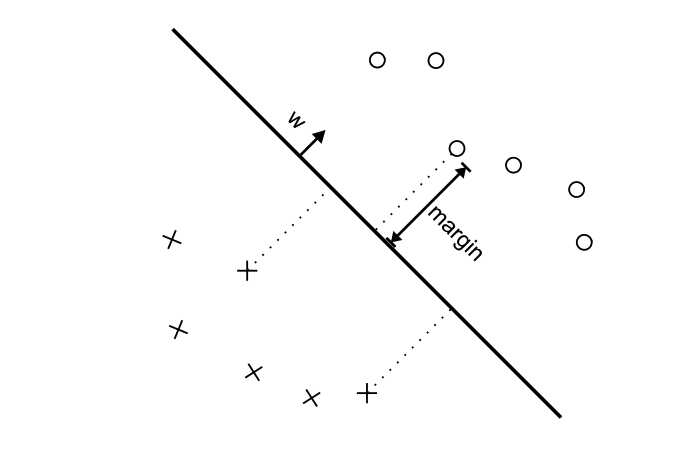
\includegraphics[width=0.5\textwidth]{linear_svm}
  \caption{Двоичная классификация SVM с линейным оператором ядра. $margin$ -- расстояние от
    гиперплоскости до каждого из классов. $w$ -- вектор нового примера, для которого делается предсказание.}\label{linear_svm}
\end{figure}

\subsubsection{Метод максимальной энтропии}
Следующей рассмотрим классификацию при помощи метода максимальной энтропии~\cite{nigam1999using}. В
случае с разбиением на два класса это использование логистической регрессии для поиска распределения
данных по классам. В отличие от наивного байесовского классификатора этот метод не
предполагает независимости признаков. Это значит, что можно использовать для предсказания признаки
разной природы, например, измерять $n$-граммы\footnote{$n$-буквенные сочетания, например, разбиение
  предложения \textbf{``Мама мыла раму.''} на 3-граммы выглядит так: \textbf{|Мам|а м|ыла| ра|му.|}} и словосочетания в сообщении одновременно.
Суть этого метода в том, что надо выбрать самую
подходящую модель, удовлетворяющую всем естественным ограничениям. Модель описывается формулой

\begin{equation}
P(c|t,\mathbf{\lambda}) = \frac{\exp\left (\sum\limits_{i=1}^N\lambda_ix_i(c,t)\right )}
{\sum\limits_{c\in\mathcal{C}} \exp\left (\sum\limits_{i=1}^N\lambda_ix_i(c,t)\right )}
\end{equation}

Здесь $c$ -- метка класса, $t$ -- рассматриваемое сообщение, $x_i(c,t)$ -- совместная
представленность $i$-ого признака в классе $c$ и в примере $t$ , $N$ --
количество признаков, $\mathbf{\lambda}$ -- вектор весов для всех
признаков: чем больше вес, тем больше значимость этого признака для классификатора. На этапе обучения
при помощи методов оптимизации вычисляется именно вектор весов признаков. При предсказании класса
для нового примера снова нужно найти такое $c^*$ из множества меток, что рассматриваемая величина $P(c|t,\mathbf{\lambda})$ будет максимальной.

\subsubsection{Сравнение работы методов на данных из Твиттера}\label{comparemeth}

Сравнение проводится на данных, собранных из Твиттера в 2009 году
\cite{go2009twitter} и расширенных собранными из Твиттера самостоятельно. Здесь мы берём текст в сыром виде, без дополнительной обработки, и передаём
алгоритму. В таблицах \ref{tab:nb}, \ref{tab:svm} и \ref{tab:maxent} представлены результаты работы
наивного байесовского классификатора, классификатора на основе метода опорных векторов и
классификатора по принципу максимальной энтропии соответственно. Алгоритмы обучались на 1000000
размеченных примеров и предсказывали результаты для 386 новых.

Чтобы оценить качество классификации, обычно используют $F1-score$ -- гармоническое среднее двух
других: $precision$ (точность) и $recall$ (полнота). На языке вероятностей можно определить эти величины следующим образом: $precision$ -- это
вероятность того, что случайно выбранный твит попал в тот класс, которому он принадлежит
на самом деле; $recall$ -- это вероятность того, что случайно выбранный твит из класса
при классификации в него и попадёт. Покажем, что значат эти величины более формально.
Пусть зафиксирован класс $c$ и есть множество всех классифицируемых твитов $\mathcal{T}$,
которое делится на два множества: $\mathcal{T}_c$ -- те, что на самом деле относятся к классу $c$,
и $\mathcal{T}\setminus\mathcal{T}_c$ -- те, у которых должны стоять другие метки.
По результатам эксперимента определяются следующие величины:
  \begin{itemize}
    \setlength{\itemsep}{1pt}%
    \setlength{\parskip}{1pt}
  \item[ ] $TP$ -- количество твитов из $\mathcal{T}_с$, которым алгоритм поставил метку $c$; \nopagebreak
  \item[ ] $FP$ -- количество твитов из $\mathcal{T}\setminus\mathcal{T}_c$, которым алгоритм поставил метку $c$; \nopagebreak
  \item[ ] $TN$ -- количество твитов из $\mathcal{T}\setminus\mathcal{T}_c$, которым алгоритм поставил метку не $c$; \nopagebreak
  \item[ ] $FN$ -- количество твитов из $\mathcal{T}_c$, которым алгоритм поставил метку не $c$.
  \end{itemize}

Для проверки работы методов используются реализации из библиотеки
Scikit-learn \cite{scikit-learn}. Для наивного байесовского классификатора предполагается, что данные
распределены по закону Бернулли.
В качестве характеристик берутся все слова, встретившиеся в обучающей выборке,
и каждый твит преобразуется в вектор из целых чисел, где
на месте $i$-ого слова ставится $0$, если слово встретилось в сообщении, и $1$, если нет.

\begin{table}[h]
    \centering
    \begin{tabular}{|c|c|c|c|c|}
      \hline
      \textbf{Метка класса} & \textbf{Precision} & \textbf{Recall} & \textbf{F1-score} &
      \textbf{Количество} \\ \hline
      -1.0&0.82&0.75&0.78&204\\ \hline
      1.0&0.74&0.82&0.78&182\\ \hline \hline
      avg / total&0.79&0.78&0.78&386\\
      \hline
    \end{tabular}
    \caption{Классификация наивным байесовским классификатором. Время обучения -- 1 с.}\label{tab:nb}
\end{table}
\begin{table}[h!]
    \centering
    \begin{tabular}{|c|c|c|c|c|}
      \hline
      \textbf{Метка класса} & \textbf{Precision} & \textbf{Recall} & \textbf{F1-score} &
      \textbf{Количество} \\ \hline
      -1.0&0.86&0.73&0.79&204\\ \hline
      1.0&0.74&0.87&0.80&182\\ \hline \hline
      avg / total&0.80&0.80&0.79&386\\
      \hline
    \end{tabular}
    \caption{Классификация методом опорных векторов. Время обучения -- 750 с.}\label{tab:svm}
\end{table}
\begin{table}[h!]
  \centering
    \begin{tabular}{|c|c|c|c|c|}
      \hline
      \textbf{Метка класса} & \textbf{Precision} & \textbf{Recall} & \textbf{F1-score} & \textbf{Количество} \\ \hline
      -1.0&0.87&0.71&0.78&204\\ \hline
      1.0&0.73&0.88&0.80&182\\ \hline \hline
      avg / total&0.80&0.79&0.79&386\\
      \hline
    \end{tabular}
    \caption{Классификация методом максимальной энтропии. Время обучения -- 437 с.}\label{tab:maxent}
\end{table}

Как уже было сказано, всего в тестовой выборке было 386 сообщений, из которых 182 были помечены
``+'', а 204 -- ``$\minus$''. Из таблиц \ref{tab:nb}, \ref{tab:svm} и \ref{tab:maxent} видно, что все методы показали
примерно одинаковую точность и полноту работы, но время обучения при этом у наивного байесовского
классификатора отличается на порядок от двух других.  Для постановки задачи, когда предсказание делается для данных из
микроблогов, время обучения при равных показателях $F1-score$ является решающим, так как меняются
темы, о которых пишут в Интернете, а значит меняются лексика и способы выражения отношения к ним --
классификатору нужно подстраиваться под эти обстоятельства, постоянно переобучаясь.

Как итог сравнения за основу для улучшения стоит взять наивный байесовский классификатор. Стоит
сказать, что для моделирования данных можно было без дополнительных усилий выбрать
и закон мультиномиального распределения. В случае с твитами это означает, что в векторе, в который этот твит
переводится, каждому слову из обучающей выборки сопоставляется количество раз, которое оно встретилось в сообщении. Когда тексты короткие, в случае с мультиномиальной моделью векторы
получаются почти всегда из $0$ и $1$, поэтому отдельно его можно и не рассматривать.

\subsection{Связанные идеи}

\subsubsection{Анализ графов слов}
Идея, предложенная в статье \cite{Colace2013}, основывается на построении графа для получения
информации о классах. Для положительных и отрицательных слов строятся два графа
соответственно. Их структуры восстанавливаются из обучающей выборки. Для присваивания метки новому
примеру предлагается использовать ещё и словарь синонимов: вероятность слова оказаться в классе учитывает количество
попаданий его самого и всех его синонимов в этот класс.

\subsubsection{Использование онтологий}
В статье \cite{Kontopoulos2013} предлагается для каждой конкретной темы строить
онтологии\footnote{Онтология -- схема области знаний.}, которые уточняют запросы, сужая все
найденные в поиске твиты до тех, в которых действительно говорится об этом объекте. Тема запроса заменяется на пару ``корень
онтологии'' и ``свойство'', например, если исходный запрос -- ``смартфон'', то
это и есть тема
онтологии, а свойствами могут быть ``android'', ``iphone'' и ``батарейка''. В этом случае вместо
одной попытки поиска будет уже три, но с более релевантной выдачей: ``смартфон android'', ``смартфон iphone'' и ``смартфон
батарейка''. При помощи коммерческой программы с закрытым исходным кодом
OpenDover\footnote{opendover.nl} авторами статьи производится дальнейший анализ окраски полученных результатов
выдачи.

Авторы статьи \cite{SaifHassanHeYulanAlani2012} предлагают использовать онтологии в момент
подготовки найденных данных к разметке. Авторы предлагают три варианта: ставить
категорию с предыдущего уровня\footnote{Для построения онтологии область знаний разбита на категории, которые сформированы в направленный
  ациклический граф. Для каждой категории, если это не корень онтологии, есть обощающая категория,
  находящаяся на предыдущем уровне.}
рядом со словом в сообщении, для которого эта категории
найдена; заменять слово на более общую категорию; рассматривать в примерах распределение слов как
условное распределение от категорий. Статья на самом деле про последний способ, потому что здесь
вероятность попадания примера в класс считается немного необычно: учитываются не только
распределения слов, но и дополнительные признаки. Точнее, от величин дополнительных признаков
зависит распределение слов в сообщении. Предложенный метод является уточнением наивного байесовского
классификатора при помощи онтологий.

\subsubsection{Расширение модели темами}
Другой взгляд на уточнение модели описан в статье \cite{Celikyilmaz2010}. Здесь предлагается
расширять стандартную модель наивного байесовского классификатора условным распределением слов, зависящим
от темы. Множество тем не фиксировано, но сказано, сколько их вообще. Перед обучением модели
говорится, что есть какое-то количество тем, по которым нужно разделить слова из обучающей выборки. Например,
вероятность встретить слово ``Шекспир'' в той же теме, что и ``Пушкин'', больше, чем в той же теме,
что и ``телефон''.
